\documentclass[10pt,aspectratio=169]{beamer}

% ============================================================
% THEME & PACKAGES
% ============================================================
\usetheme{Madrid}
\usecolortheme{dolphin}
\useinnertheme{rounded}
\useoutertheme{shadow}

\usepackage[T2A]{fontenc}
\usepackage[utf8]{inputenc}
\usepackage[english]{babel}
\usepackage{amsmath,amssymb}
\usepackage{graphicx}
\usepackage{tikz}
\usepackage{colortbl}
\usepackage{booktabs}
\usepackage{hyperref}
\usepackage{multicol}
\usepackage{tabularx}
\usepackage{array}
\usepackage{ragged2e}

% Custom colors
\definecolor{deepblue}{RGB}{26,32,68}
\definecolor{accentblue}{RGB}{59,130,246}
\definecolor{accentgreen}{RGB}{16,185,129}
\definecolor{accentorange}{RGB}{245,158,11}
\definecolor{accentred}{RGB}{239,68,68}
\definecolor{lightgray}{RGB}{241,245,249}
\definecolor{darktext}{RGB}{30,41,59}

\setbeamercolor{title}{fg=white}
\setbeamercolor{frametitle}{bg=deepblue,fg=white}
\setbeamercolor{structure}{fg=accentblue}
\setbeamercolor{normal text}{fg=darktext}
\setbeamercolor{itemize item}{fg=accentblue}
\setbeamercolor{itemize subitem}{fg=accentblue}
\setbeamercolor{block title}{fg=white,bg=accentblue}
\setbeamercolor{block body}{bg=lightgray,fg=darktext}
\setbeamercolor{alerted text}{fg=accentred}

\setbeamertemplate{navigation symbols}{}
\setbeamertemplate{footline}{
    \leavevmode%
    \hbox{%
    \begin{beamercolorbox}[wd=.95\paperwidth,ht=2.5ex,dp=1ex,right]{date in head/foot}%
        \usebeamerfont{date in head/foot}\insertframenumber{} / \inserttotalframenumber\hspace*{2ex}
    \end{beamercolorbox}}%
    \vskip0pt%
}

% ============================================================
% TITLE PAGE
% ============================================================
\title[Deadline Optimizer]{\Large\textbf{Assignment Deadline Optimizer}}
\subtitle{\small AI-powered personal deadline tracker}
\author[I. Kostina]{
    \texorpdfstring{
        \textbf{Irina Kostina} \\[2pt]
        \href{mailto:i.kostina@innopolis.university}{i.kostina@innopolis.university} \\[2pt]
        Group CSE-04
    }{Irina Kostina -- i.kostina@innopolis.university -- Group CSE-04}
}
\institute[Innopolis University]{Innopolis University}
\date{Lab 9 -- Hackathon \quad 2026}

% ============================================================
% DOCUMENT
% ============================================================
\begin{document}

% --- SLIDE 1: TITLE ---
{
\setbeamertemplate{background canvas}{
    \begin{tikzpicture}[remember picture,overlay]
        \fill[deepblue] (current page.south west) rectangle (current page.north east);
        \fill[accentblue,opacity=0.1] (current page.north east) circle (5cm);
        \fill[accentgreen,opacity=0.08] (current page.south west) circle (6cm);
        \fill[accentorange,opacity=0.05] (current page.north west) circle (4cm);
    \end{tikzpicture}
}
\begin{frame}
    \vfill
    \begin{center}
        {\Huge\color{white}\textbf{Assignment Deadline Optimizer}} \\[12pt]
        {\large\color{accentblue!80!white} AI-powered personal deadline tracker that analyzes workload, prioritizes tasks, and tells you exactly what to work on and when} \\[24pt]
        \rule{0.5\textwidth}{0.5pt} \\[12pt]
        {\color{white}
        \textbf{Irina Kostina} \\
        \href{mailto:i.kostina@innopolis.university}{\color{accentblue!70!white}i.kostina@innopolis.university} \\
        Group CSE-04 \\[8pt]
        \color{gray} Innopolis University \quad|\quad Lab 9 -- Hackathon \quad|\quad 2026
        }
    \end{center}
    \vfill
\end{frame}
}

% --- SLIDE 2: CONTEXT ---
{
\setbeamertemplate{background canvas}{
    \begin{tikzpicture}[remember picture,overlay]
        \fill[lightgray!30] (current page.south west) rectangle (current page.north east);
    \end{tikzpicture}
}
\begin{frame}{Context}
    \vspace{4pt}

    \begin{block}{End User}
        University students managing 4--5 courses per semester, each with multiple assignments, labs, and exams with overlapping deadlines.
    \end{block}

    \begin{alertblock}{Problem}
        Students face 4--5 overlapping deadlines every week, don't know where to start, panic, and end up submitting late or producing low-quality work.
    \end{alertblock}

    \begin{block}{Product Idea}
        \textbf{AI-powered personal deadline tracker} that analyzes your workload, prioritizes tasks by urgency and complexity, and tells you \emph{exactly what to work on and when}.
    \end{block}

    \vspace{6pt}
    \begin{center}
        \setlength{\tabcolsep}{10pt}
        \renewcommand{\arraystretch}{1.2}
        \begin{tabular}{c c c c}
            \raisebox{-1pt}{\textcolor{deepblue}{\Huge $\langle/\rangle$}} &
            \raisebox{-1pt}{\textcolor{accentgreen}{\Huge $\dblozenge$}} &
            \raisebox{-1pt}{\textcolor{accentblue}{\Huge $\boxplus$}} &
            \raisebox{-1pt}{\textcolor{accentorange}{\Huge $\odot$}} \\[4pt]
            FastAPI & PostgreSQL & React SPA & MCP Agent \\
            Backend & Database & Frontend & Nanobot
        \end{tabular}
    \end{center}
\end{frame}
}

% --- SLIDE 3: IMPLEMENTATION ---
{
\setbeamertemplate{background canvas}{
    \begin{tikzpicture}[remember picture,overlay]
        \fill[lightgray!30] (current page.south west) rectangle (current page.north east);
    \end{tikzpicture}
}
\begin{frame}{Implementation}
    \vspace{2pt}

    \begin{columns}[T]
        \begin{column}{0.48\textwidth}
            \textcolor{accentblue}{\textbf{\large Version 1 -- Core Feature}}
            \vspace{4pt}
            \begin{itemize}
                \itemsep 4pt
                \item Priority scoring algorithm: \emph{urgency + weight + status}
                \item AI recommendations per task
                \item Risk levels: low / medium / high / critical
                \item Conflict detection for overlapping deadlines
                \item Progress tracking per course
            \end{itemize}
        \end{column}
        \begin{column}{0.48\textwidth}
            \textcolor{accentgreen}{\textbf{\large Version 2 -- Improvements}}
            \vspace{4pt}
            \begin{itemize}
                \itemsep 4pt
                \item Full CRUD via web UI (create/delete deadlines)
                \item Management panel with forms
                \item Dashboard with charts (Chart.js)
                \item MCP server -- 7 tools for AI agent
                \item Docker Compose -- 8 services
                \item OpenTelemetry observability
            \end{itemize}
        \end{column}
    \end{columns}

    \vspace{8pt}
    \begin{block}{TA Feedback Addressed}
        Added management panel for CRUD operations; improved conflict warnings visibility in UI; added productivity statistics endpoint; created comprehensive test suite (58 tests passing).
    \end{block}

    \vspace{4pt}
    \begin{center}
        \textcolor{deepblue}{\textbf{Tech Stack:}} \quad
        \setlength{\tabcolsep}{6pt}
        \begin{tabular}{c c c c c}
            \colorbox{accentblue!15}{\texttt{FastAPI}} &
            \colorbox{accentgreen!15}{\texttt{PostgreSQL}} &
            \colorbox{accentorange!15}{\texttt{React+TS}} &
            \colorbox{accentred!15}{\texttt{MCP}} &
            \colorbox{deepblue!15}{\texttt{Docker}}
        \end{tabular}
    \end{center}
\end{frame}
}

% --- SLIDE 4: DEMO ---
{
\setbeamertemplate{background canvas}{
    \begin{tikzpicture}[remember picture,overlay]
        \fill[lightgray!30] (current page.south west) rectangle (current page.north east);
        \draw[accentblue!40, line width=1pt, rounded corners=8pt]
            (1.2,1.2) rectangle (11.8,5.5);
    \end{tikzpicture}
}
\begin{frame}{Demo}
    \vspace{2pt}

    \begin{center}
        \textcolor{accentred}{\textbf{Pre-recorded video demonstration of Version 2 with voice-over ({$\le$} 2 minutes)}}
    \end{center}

    \vspace{6pt}
    \begin{center}
        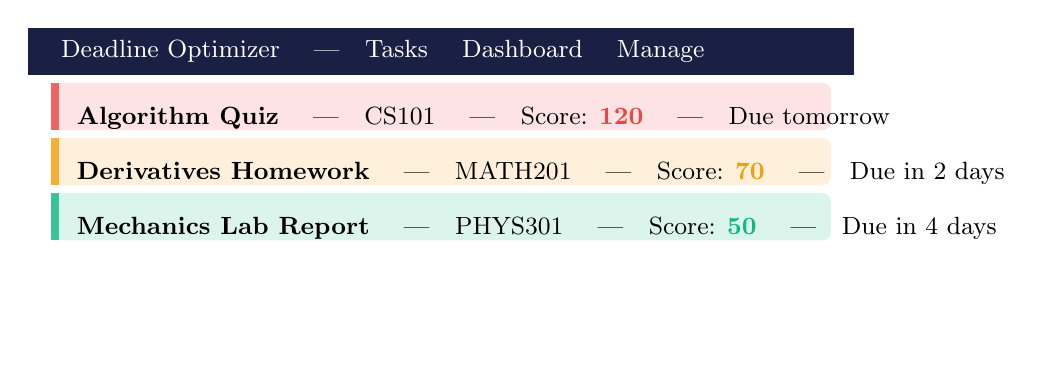
\begin{tikzpicture}
            \fill[white,rounded corners=6pt] (0,0) rectangle (10.5,4);
            \fill[deepblue] (0,3.4) rectangle (10.5,4);
            \node[white,right] at (0.3,3.7) {\small Deadline Optimizer \quad|\quad Tasks \quad Dashboard \quad Manage};
            \fill[accentred!15,rounded corners=3pt] (0.3,2.7) rectangle (10.2,3.3);
            \fill[accentred,opacity=0.8] (0.3,2.7) rectangle (0.4,3.3);
            \node[right,align=left] at (0.5,2.85) {\small \textbf{Algorithm Quiz} \quad|\quad CS101 \quad|\quad Score: \textcolor{accentred}{\textbf{120}} \quad|\quad Due tomorrow};
            \fill[accentorange!15,rounded corners=3pt] (0.3,2.0) rectangle (10.2,2.6);
            \fill[accentorange,opacity=0.8] (0.3,2.0) rectangle (0.4,2.6);
            \node[right,align=left] at (0.5,2.15) {\small \textbf{Derivatives Homework} \quad|\quad MATH201 \quad|\quad Score: \textcolor{accentorange}{\textbf{70}} \quad|\quad Due in 2 days};
            \fill[accentgreen!15,rounded corners=3pt] (0.3,1.3) rectangle (10.2,1.9);
            \fill[accentgreen,opacity=0.8] (0.3,1.3) rectangle (0.4,1.9);
            \node[right,align=left] at (0.5,1.45) {\small \textbf{Mechanics Lab Report} \quad|\quad PHYS301 \quad|\quad Score: \textcolor{accentgreen}{\textbf{50}} \quad|\quad Due in 4 days};
        \end{tikzpicture}
    \end{center}

    \vspace{8pt}
    \begin{columns}[T]
        \begin{column}{0.23\textwidth}
            \begin{center}
                {\Huge \textcolor{accentblue}{\textbf{5}}} \\[2pt]
                \small Courses
            \end{center}
        \end{column}
        \begin{column}{0.23\textwidth}
            \begin{center}
                {\Huge \textcolor{accentgreen}{\textbf{12}}} \\[2pt]
                \small Assignments
            \end{center}
        \end{column}
        \begin{column}{0.23\textwidth}
            \begin{center}
                {\Huge \textcolor{accentorange}{\textbf{37}}} \\[2pt]
                \small Unit Tests
            \end{center}
        \end{column}
        \begin{column}{0.23\textwidth}
            \begin{center}
                {\Huge \textcolor{accentred}{\textbf{7}}} \\[2pt]
                \small MCP Tools
            \end{center}
        \end{column}
    \end{columns}

    \vspace{4pt}
    \begin{center}
        \footnotesize \textcolor{gray}{Video file: \texttt{https://drive.google.com/file/d/1fXM1kWkiodFm7xbjYeh_VISY3W8bfFa-/view?usp=sharing} -- attached separately}
    \end{center}
\end{frame}
}

% --- SLIDE 5: LINKS ---
{
\setbeamertemplate{background canvas}{
    \begin{tikzpicture}[remember picture,overlay]
        \fill[deepblue] (current page.south west) rectangle (current page.north east);
        \fill[accentblue,opacity=0.08] (current page.north east) circle (5cm);
        \fill[accentgreen,opacity=0.06] (current page.south west) circle (6cm);
    \end{tikzpicture}
}
\begin{frame}{Links}
    \vspace{6pt}

    \begin{columns}[T]
        \begin{column}{0.45\textwidth}
            \begin{block}{GitHub Repository}
                \centering
                \href{https://github.com/Rena-ln/se-toolkit-lab-9}{
                    \textcolor{accentblue}{\texttt{github.com/Rena-ln/}} \\
                    \textcolor{accentblue}{\texttt{se-toolkit-lab-9}}
                } \\[12pt]
                
\includegraphics[width=3cm]{qr-code1.png}
            \end{block}
        \end{column}
        \begin{column}{0.45\textwidth}
            \begin{block}{Deployed Product}
                \centering
                \href{http://10.93.24.215:8080/}{
                    \textcolor{accentgreen}{\texttt{http://10.93.24.215:8080/}}
                } \\[12pt]
                
\includegraphics[width=3cm]{qr-code.png}
            \end{block}
        \end{column}
    \end{columns}

    \vspace{8pt}
    \begin{center}
        \begin{tabular}{c c c}
            \colorbox{white}{\texttt{API Key: dev-api-key-change-in-production}} &
            \quad &
            \colorbox{accentblue!20}{\texttt{MIT License}}
        \end{tabular}
    \end{center}

    \vspace{12pt}
    \begin{center}
        {\color{white}
        \textbf{Irina Kostina} \quad|\quad
        \href{mailto:i.kostina@innopolis.university}{i.kostina@innopolis.university} \quad|\quad
        CSE-04 \quad|\quad
        Innopolis University
        }
    \end{center}
\end{frame}
}

\end{document}
